\chapter{le concept de la signature électronique}
	\section*{Introduction}
		Dans ce chapitre nous allons mettre en évidence les concepts générales sur la signature électronique. Ensuite nous donnerons une idée générale sur la procédure ou la mécanisme de la signature électronique dans sa vue globale et les différentes méthodes peuvent intervenir pour la rendre encore plus sûre. Donc nous allons présentés premièrement les généralités sur la signature numérique en soulignant son rôle ainsi que les différents technologie qui interviennent.
	
	\section{Généralités sur la signature électronique}
	Pour mieux savoir ce que c'est une signature électronique, nous parlerons de ce qu'on entend par signature. \textbf{C'est  quoi une signature ?} 
		\subsection{Signature}
		
		 	\begin{figure}[H]
		 		\centering
		 		
\includegraphics[width=17cm, height=5cm]{../imgs/signature}
		 		\caption{Représentation graphique d'une signature}
		 		\label{signature}
		 	\end{figure}
			\subsubsection{Définition}
				La signature est le graphisme par lequel une personne s'identifie dans un acte et, par lequel elle exprime son approbation au contenu de ce document. La validité de tout engagement est subordonné à l'existence de cette signature manuscrite qui confère au document sa force probatoire.
				
				La signature peut également être le révélateur d'une maladie ou d'un acte (parfois criminel) commis par un individu, dans le sens où elle permet d'identifier clairement la maladie, ou l'auteur de l'acte en question. Une signature a donc pour but de permettre une identification. Le paraphe est la marque visuelle abrégée de la signature complète.
			
			    La figure \ref{signature} est la représentation graphique d'une signature dite manuscrite, son utilisation est faite soit sur les documents physiques soit sur les document numériques de façon clair c'est à visible à l'oeil nue, c'est qui est exposé au faux, falsification etc, des signatures d'autrui.
			\subsubsection{Faux et usage de faux en signatures.}
			    Imiter la signature d’un individu sur un document, même si la signature imitée ne ressemble en rien la signature officielle de la personne lésée, peut constituer un délit de faux et usage de faux et d’usurpation d’identité, ainsi que d’autres délits répertoriés dans le code civil ou pénal : arnaque, escroquerie, vol de biens, de droits, vol d’identité, détournement de fonds, d’héritage, etc.
			    
			    Même avec autorisation verbale ou procuration écrite, le signataire doit impérativement y apposer sa propre signature sans imiter celle de la personne ayant autorisé l’acte. Autrement, on parlerait d’imitation, d’usurpation de signature.

                Mais le faux en signatures le plus habituelle se fait sans autorisation ni procuration, tout simplement par abus de confiance, par abus de faiblesse.

                C’est le cas des contrats de crédits en ligne signés à la place et à l’écart des conjoints, les chèques bancaires signés à la place et majeurs, souvent placés sous tutelle, les documents administratifs signés à la place d’un proche pour accélérer les procédures ou le tenir à l’écart, etc.

                Les procédés utilisés par les faussaires sont nombreux, étant souvent très difficiles à identifier. On peut évoquer l’imitation manuelle, plus ou moins réussie, le faux par décalquage, la photo-composition physique ou numérique, ainsi que l’imitation de fantaisie, ou le résultat ne comporte aucune ressemblance par rapport à la vraie signature de la victime.
                
                On peut constater que les risques de falsification de signature manuscrite sont énormes, pour palier à ces problèmes on a une autre manière de signer les documents numériques de façon totalement transparente. Bien sûr il s'agit de la signature numérique.
                
	    \subsection{Signature électronique}
			    À présent voyons voir ce que c'est une signature numérique(dite aussi électronique).
			    	
		    	\begin{figure}[H]
		 	    	\centering
		 	    	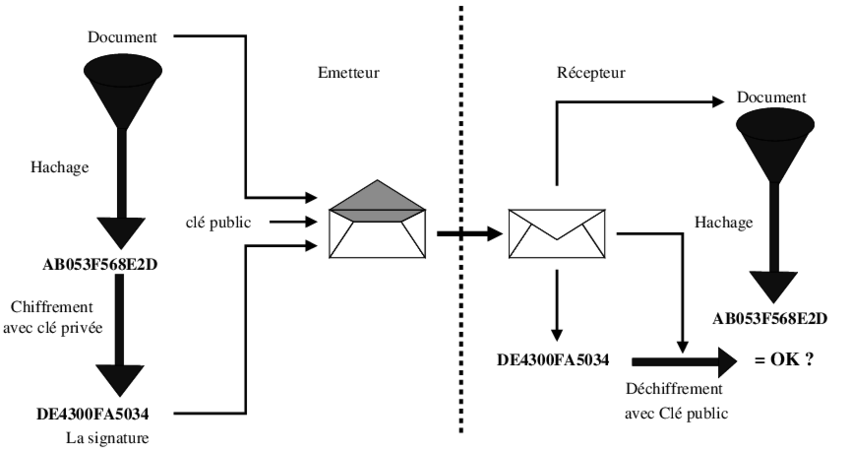
\includegraphics[width=16cm, height=5cm]{../imgs/signnum.png}
		 	    	\caption{Schéma d'utilisation de la signature numérique }
		 	    	{Source d'image:\footnote{https://www.researchgate.net/figure/Schema-dutilisation-de-la-signature-numerique-La-methode-nest-pas-sur-et-le-contenu}}
		 	    	\label{signum}
		    	\end{figure}
		    	
		    \subsubsection{Qu’est-ce que la signature électronique ?}
		        Cette question, qui semble pourtant basique, est au coeur du débat. Car avant de l’adopter, encore faut-il savoir de quoi il s’agit concrètement. Avant toute chose, il est important de comprendre ce que la signature électronique n’est pas, et surtout de couper court à certaines croyances populaires : en l’occurrence, la signature électronique n’est pas un « scan » de la signature manuscrite\cite{certeurope}.Ceci étant précisé, \textbf{ qu’est-ce que la signature électronique alors ?}
		    	
			    
			\subsubsection{Définitions}
			    La signature électronique (dite aussi signature numérique) est un processus, utilisant des mécanismes de cryptologie, permettant de garantir l'intégrité d'un document électronique et d'en authentifier l'auteur, par analogie avec la signature manuscrite d'un document papier.\\
			    
			    La signature numérique constitue la forme de signature électronique la plus avancée et sécurisée. Vous pouvez l’utiliser pour vous conformer aux dispositions réglementaires et juridiques les plus strictes, car elle offre les niveaux de garantie les plus élevés sur l'identité des signataires et l'authenticité des documents qu'ils signent.\\
			    
                Les signatures numériques utilisent un identifiant numérique basé sur un certificat délivré par une autorité de certification ou un prestataire de services de confiance accrédité. Ainsi, lorsque vous signez numériquement un document, votre identité vous est associée de manière exclusive, la signature est liée au document par cryptage, et tout peut être vérifié à l’aide d’une technologie sous-jacente appelée l'infrastructure à clé publique.\\
                
                 En résumé, la signature électronique est un procédé technique dans lequel une personne (le signataire) appose son accord à valeur juridique sur un document électronique. Dans un cas (électronique) comme dans l’autre (manuscrite), il y a donc réunion de 3 items : le document, le signataire et l’outil de signature\cite{certeurope}.\\
                 
                 Ce dernier point représente généralement la plus grande difficulté de compréhension au non-initié. Car si l’outil nécessaire à la signature manuscrite n’est ni plus ni moins qu’un stylo, les outils de signature électronique sont multiples, autant que les moyens techniques nécessaires à leur réalisation. Concrètement, il s’agit dans la majorité des cas d’un certificat numérique porté sur différents supports (carte à puce, clé USB, carte d’identité, PC, smartphone, etc.) et qui a pour fonction d’identifier le signataire d’une part, et de sceller le document pour en garantir l’intégrité d’autre part.
                 
                
            \subsubsection{La signature numérique a-t-elle la même valeur juridique que la signature manuscrite ?}
            
                La signature électronique a été introduite dans le droit français par la loi du 13 mars 2000\cite{signapp}. Elle dispose des mêmes prérogatives et engage le consentement du signataire de la même façon que la signature manuscrite, sous réserve de « l’usage d’un procédé fiable d’identification garantissant son lien avec l’acte auquel elle s’attache », selon l’article 1367 du Code Civil.\\
                
                Mais elle va encore plus loin que la signature manuscrite : en scellant l’ensemble du document lors de son apposition, elle en garantit l’intégrité, c’est-à-dire l’état précis, au moment de l’engagement du consentement par le signataire. Un peu comme si l’on paraphait chaque lettre ou chaque ponctuation d’un document papier ! En d’autres termes, la signature électronique profite non seulement de la même valeur juridique que la signature manuscrite, mais elle est aussi beaucoup plus sécurisante pour toutes les parties.
                
            
			    
			    
			    
			    
			\subsubsection{Rôle de signature électronique}
			    Typiquement, dans un monde où n’importe quel cybercriminel\footnote{Homme qui commet un crime à l'aide d'outils informatiques, notamment en piratant des données existantes sur Internet afin d'obtenir illégalement de l'argent ou un quelconque profit.} peut usurper l’adresse émail d’un contact et envoyer des courriers malveillants et des documents infectés en son nom, la signature électronique joue un rôle clé dans la sécurisation des échanges. Si un contact signe systématiquement tous les courriers qu’il envoie, la réception d’un courrier non signé de sa part est un signe d’usurpation. D’une façon similaire, signer un document permet d’en assurer l’authenticité et l’origine puisque l’opération est datée, que le créateur est authentifié et que la non-répudiation ne permet pas d’en modifier l’origine.\\

                Mais la signature d’un document ne cherche pas uniquement à authentifier son créateur ou son expéditeur. Elle garantit aussi l’intégrité de ce document. Et cette garantie devient de plus en plus nécessaire dans un monde connecté où les malwares\footnote{Le malware est la contraction des termes anglais malicious et software. Il désigne un logiciel malveillant s'attaquant aux ordinateurs, terminaux mobiles et objets connectés} peuvent modifier des documents et où des cybercriminels peuvent être payés, par des concurrents par exemple, pour venir altérer à votre insu des documents et vous mettre en situation délicate.\\
                Les signes de validation apposés sur un document existent depuis des millénaires (exemple : les sceaux). En France, c’est une ordonnance royale de 1554 qui a institué l'apposition de la marque autographe du nom propre sur les actes notariés\cite{signrole}.\\
                
                La signature est présentée comme indispensable pour authentifier un document. Elle permet au lecteur d’identifier la personne et l’organisme qui l’a émis. Elle apporte de la confiance dans l’environnement numérique, la confiance dans le signataire et dans le contenu de l’information.\\
                
                La signature électronique est un mécanisme permettant de garantir l'intégrité d'un document électronique et d'en authentifier l'auteur, par analogie avec la signature manuscrite d'un document papier.\\
                
                Cependant elle se différencie de la signature écrite par le fait qu'elle n'est pas visuelle : l’identification ne repose sur aucun élément graphique.
                
                         \subsubsection*{Comment la signature électronique fonctionne ?}
                
                    Concrètement suivant la Figure \ref{signum} , on commence par générer une empreinte grâce au fonction mathématique dite de hachage ou encore cette empreinte est appelée le condensé du message que l'on souhaite envoyer. Ensuite on chiffre le l'empreinte par la clé privée de l'émetteur. Le couple message original et le chiffré de l'empreinte constitue le message signer par l'émetteur. Cette empreinte servira de vérifier l'intégrité de message source.\\
                
                Du côté du destinataire, une fois qu'il a reçu le message signer c'est à dire le chiffré de empreinte et le message en clair, il procède de la même manière en générant l'empreinte du message clair en utilisant la même fonction mathématique de hachage, ensuite il décrypte l'empreinte reçu et il compare les deux hachés, s'il y'a égalité alors le message n'a pas été altéré sinon c'est dire que les deux hachés ne correspondent pas alors le message à été altéré durant son parcours vers le destinataire.
                
	\section{Cryptographie}
		\subsection{Terminologie}
			\begin{itemize}
				\item La \textbf{Cryptographie} est la science des messages secrets. Elle se décompose en deux disciplines : la cryptographie et la cryptanalyse. Dans la figure ci-dessous on voit que la cryptographie est le centre de débat de la cryptologie, ce qui fait que dans cette section on va seulement nous intéressé à la cryptographie.
			\begin{figure}[H]
                                \centering
                                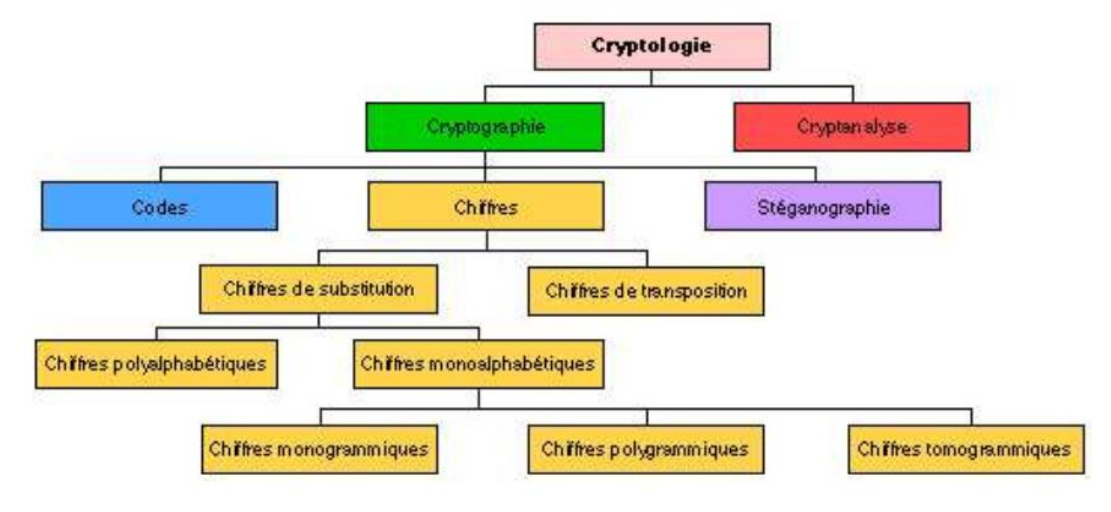
\includegraphics[width=16cm, height=9cm]{../imgs/discplinecrypto.png}
                                \caption{L'arbre hiérarchique de la cryptologie }
                                \label{discplinecrypto}
                        \end{figure}
				\item \textbf{Cryptographie} : Art de transformer un message claire en un message inintelligible. Cependant, on utilise souvent le cryptographie comme synonyme de cryptographie.
				\item \textbf{Cryptanalyse}: Art d'analyser un message chiffré afin de le décrypter. On parle aussi de décryptement.
				\item \textbf{Chiffre} (ou chiffrement) : Ensemble de procédés et ensemble de symboles(lettres, nombres, signes, etc.) employés pour remplacer les lettres du message à chiffrer. Bien souvent appelé cryptage, un mot qui provient d'anglicisme "encryption".

				\item \textbf{Code} Ensemble de procédés et ensemble de symboles(lettres,nombres, signes, etc.) employés pour remplacer les mots du message à coder.
				\item \textbf{Stéganographie :} Branche particulière de la cryptographie qui consiste non pas à rendre le message inintelligible, mais à le camoufler dans un support (texte, image, etc.) de manière à masquer sa présence.
				\item \textbf{Déchiffrement :} Opération inverse du chiffrement : obtenir la version originale d'un message qui a été précédemment chiffré en connaissant la méthode de chiffrement et les clefs.
				\item \textbf{Décryenumerateptement} (ou décryptage) : Restauration des données qui avaient été chiffrées à leur état premier, sans disposer des clefs théoriquement nécessaires.
				\item \textbf{Texte en clair : } c'est le message à protéger \cite{crypto2,}.
				\item \textbf{Texte chiffré : } c'est le résultat du chiffrement du texte clair.
				\end{itemize}
				
			\subsection{Buts de la cryptographie}
				Globalement, la cryptographie permet de résoudre quatre problèmes différents :
				\begin{enumerate}
					\item  \textbf{La confidentialité: } Le texte chiffré ne doit être lisible que par les destinataires légitimes. Il ne doit pas pouvoir être lu par un intrus.
					\item \textbf{L'authentification : }Le destinataire d'un message doit pouvoir s'assurer de son origine. Un intrus ne doit pas être capable de se faire passer pour quelqu'un d'autre.
					\item \textbf{L'intégrité : } Le destinaire d'un message doit pouvoir vérifier que celui-ci n'a pas été modifié en chemin. Un intrus ne doit pas être capable de faire passer un faux message pour légitime.
					\item \textbf{La non répudiation : } Un expéditeur ne doit pas pouvoir , par la suite, nier à tort avoir envoyé un message ainsi que le destinataire ne doit pas pouvoir nier à tort avoir reçu un message.
				\end{enumerate}
				
				\paragraph{Note}
				Il ne faut pas confondre \textbf{cryptographie} et \textbf{codage}. En effet, la cryptographie va s'attacher à cacher le sens d'un texte ;Le codage quant à lui s'attache à modifier le texte de façon à utiliser un support particulier. Ainsi par exemple, il existe le code \textbf{Morse} qui transforme les chiffres et lettres d'un texte en une succession de traits et de points afin de pouvoir utiliser le support télégraphique. Il existe aussi le code \textbf{ASCII} qui transforme les caractères en valeurs codées sur 8
bits (de 0 à 255) pour utiliser les supports informatiques. Il n'y a strictement rien de secret dans un codage.
			\subsubsection{Alice, Bernard et autres}
				Traditionnellement, pour illustrer les protocoles, on parle de communication entre des personnes fictives. Pour la cryptographie, par convention, ces personnes sont :
				\begin{center}
					\begin{tabular}{|l|l|l|}
						\hline
						\rowcolor{gray!40}Français&Anglais&Rôle\\\hline
						Alice & Alice & Alice veut envoyer un message à Bob \\\hline
						Bob & Bob & Bob communique avec Alice \\\hline
						Christine & Carol & S'il faut un $3^{ème}$ pour communiquer avec Alice et Bob c'est Christine\\\hline
						David & Dave &  S'il faut un $4^{ème}$ pour communiquer avec Alice et Bob c'est David\\\hline
						... & ... & ...\\
					
					\end{tabular}
				\end{center}
				
				
				
				
				
				
				
				
				
				
				
				
				
				
				
				
				
				
				
				
				
				
				
				
				
				
		\subsection{Cryptographie symétrique}
			
		\subsection{Cryptographie asymétrique}
	
	\section{Infrastructure à clé publique}
	
			
\section*{Conclusion}
